\documentclass{elsarticle}

\usepackage[letterpaper, margin=1in]{geometry}
\usepackage{titlesec}
\usepackage{enumitem}
\usepackage{graphicx,amsmath, amssymb, amsthm, amsfonts,subcaption}
\usepackage[usenames, dvipsnames]{xcolor}
\usepackage{float}
\usepackage{tikz}
\usepackage{xspace} 

\newcommand{\iqspc}{IQS-PC\xspace}

\newcommand{\fix}{\textsquare}
\newcommand{\working}{$\boxdot$}
\newcommand{\nofix}{?}
\newcommand{\done}{\checkmark}

%\newcommand{\easy}[1]{\textcolor{ForestGreen}{#1}}
%\newcommand{\medm}[1]{\textcolor{BurntOrange}{#1}}
%\newcommand{\hard}[1]{\textcolor{Red}{#1}}
\newcommand{\easy}[1]{\textbf{\textit{#1}}}
\newcommand{\medm}[1]{\textbf{\textit{#1}}}
\newcommand{\hard}[1]{\textbf{\textit{#1}}}

\begin{document}

\section*{Major Issues}

\begin{itemize}

\item[\done] \medm{ Justify page 8: ``we expect temperature to be more rapidly varying than the shape but less so than the amplitude" }
\begin{itemize}
\item Page 9: ``This idea stems from the fact that in a adiabatic temperature model, the temperature's spatial variation follows the neutron flux shape, while the temperature amplitude follows the flux amplitude. Because of the heat capacity of the fuel, the temperature amplitude is more slowly varying in time than the heat inflow from the flux amplitude, while still considerably faster than the time variance of the flux shape. This logic is empirically defended in the results of Section 5."
\end{itemize}

\item[\done] \easy{ Justify page 5: ``Using IQS, one expects the time dependence of the shape to be weaker than that of the flux itself, this allowing for larger time step sizes in updating the shape". }
\begin{itemize}
\item Page 5: References [1] as justification for this statement.
\end{itemize}

\item[\working] \medm{  Results are often just stated and not discussed, e.g. page 19 ``It also shows that traditional IQS performed better with large etol, while IQS-PC was better with smaller etol". The statement simply bloats the manuscripts; discuss the reasons and implications or remove it. Another example is page 15, ``However, switching the precursors solve to be performed semi-analytically…".  In this case, the authors should take the time to discuss the implications of this finding. }
\begin{itemize}
\item Page 16: Added ``This result implies that uniqueness of the shape and amplitude can only be maintained with a consistent treatment of precursor term in the shape equation."
\item Page 18: Removed ``This illustrates that IQS can yield a much more accurate solution, even at a significantly larger time step than the implicit flux discretization."
\item Page 20: Added ``These convergence results are consistent with the hypothesis that the performance of IQS is highly dependent on the spatial coupling of the flux."
\item Page 20: Added ``This observation implies that the time adaptive options must be chosen differently when applied to a solver for shape versus a solver for flux."
\end{itemize}

\item[\done] \medm{ For the comparison of LRA and TREAT results, the efficiency [how accurate can you be given a fixed execution time or given an accuracy how much execution time do you need] is a very important quantity; the authors discuss it for LRA and TREAT. However, the authors first present results for the errors and then runtime results. Then they try to synthesize efficiency by comparing different cases that have different runtimes and different errors, e.g. page 23 right before Table 5 ``IQS-PC shows and error less than implicit discretization at delta t = 0.002, signifying …". I suggest the authors create error vs. execution time plots for different cases and based on these curves discuss efficiency. The manner efficiency is discussed is very confusing and not very useful for the reader. }
\begin{itemize}
\item Page 24: ``Fig. 17 visualizes the dependence of run-time on error. This figure shows that IQS and IQS P-C generally has a lower run-time for certain error than implicit discretization. Furthermore, note that the slopes on the right half of the \iqspc runs are shallower than the implicit discretization slope. This shows that by adding more temperature updates, within the 1-4 temperature updates region, \iqspc suffers a smaller increase in run-time for a decrease in error. However, the error in the shape function saturates the full error after adding more than four updates, leading to an inelastic dependence on run-time. "
\end{itemize}
%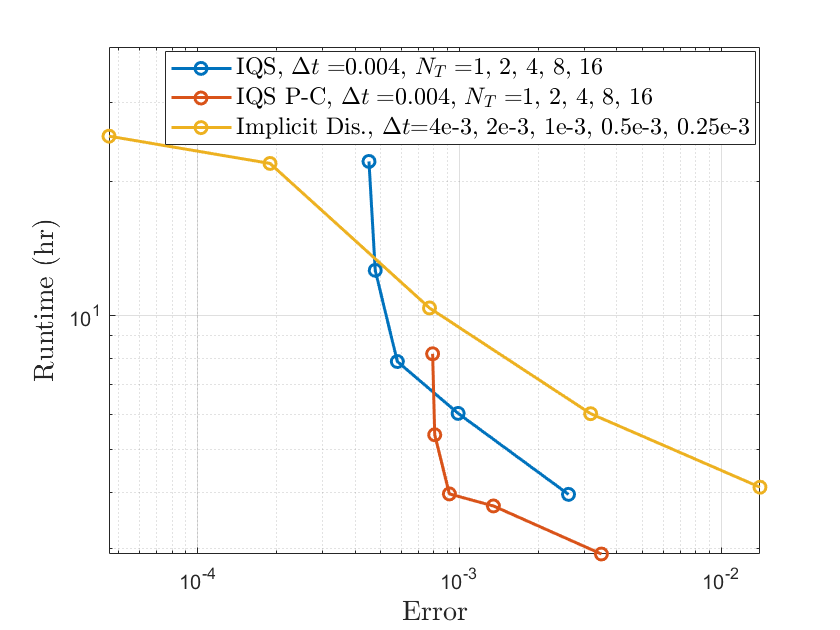
\includegraphics[height=3in]{figures/lra_rt_vs_err.png}


\item[\done] \easy{ In the results section, Error is sometimes used without introducing it, e.g. page 25, ``Table 9 shows the error ….". Further ``Error" is often used as y-label in plots., e.g. in the discussion of Figure 10 in which ``convergence results" are presented; the sentence is not clear in this context because it was not stated if this is iterative convergence or convergence to the right solution as the time step is reduced. In some instances error is defined but it is tedious for the reader to find the corresponding passage in the text, figures, or tables. }
\begin{itemize}
\item Page 17-25: Included an explicit definition of error in each of the plots and tables
\end{itemize}

\item[\done] \hard{ LRA and TREAT only compare errors computed with the peak powers. Peak powers are an integral quantity and may favor IQS over spatial kinetics. The authors should also compare power distributions or similar distributed quantities. }
\begin{itemize}
\item Page 24-26: ``All the values for error in this section are errors in the globally integrated flux. However, it is noteworthy to compare the spatial dependence of error. Fig. 18 shows the difference in normalized power at each block of the LRA geometry for each method. The resulting spatially dependent error is in general an order of magnitude lower for IQS and IQS P-C than implicit discretization. This observation corresponds well with the globally integrated flux errors shown in Tables 6-8."
\end{itemize}
%\resizebox{\textwidth}{!}{%
%\begin{tikzpicture}[every node/.style = {font=\normalsize}]
%\node[inner sep=0pt, anchor=south](fig) at (0,0) {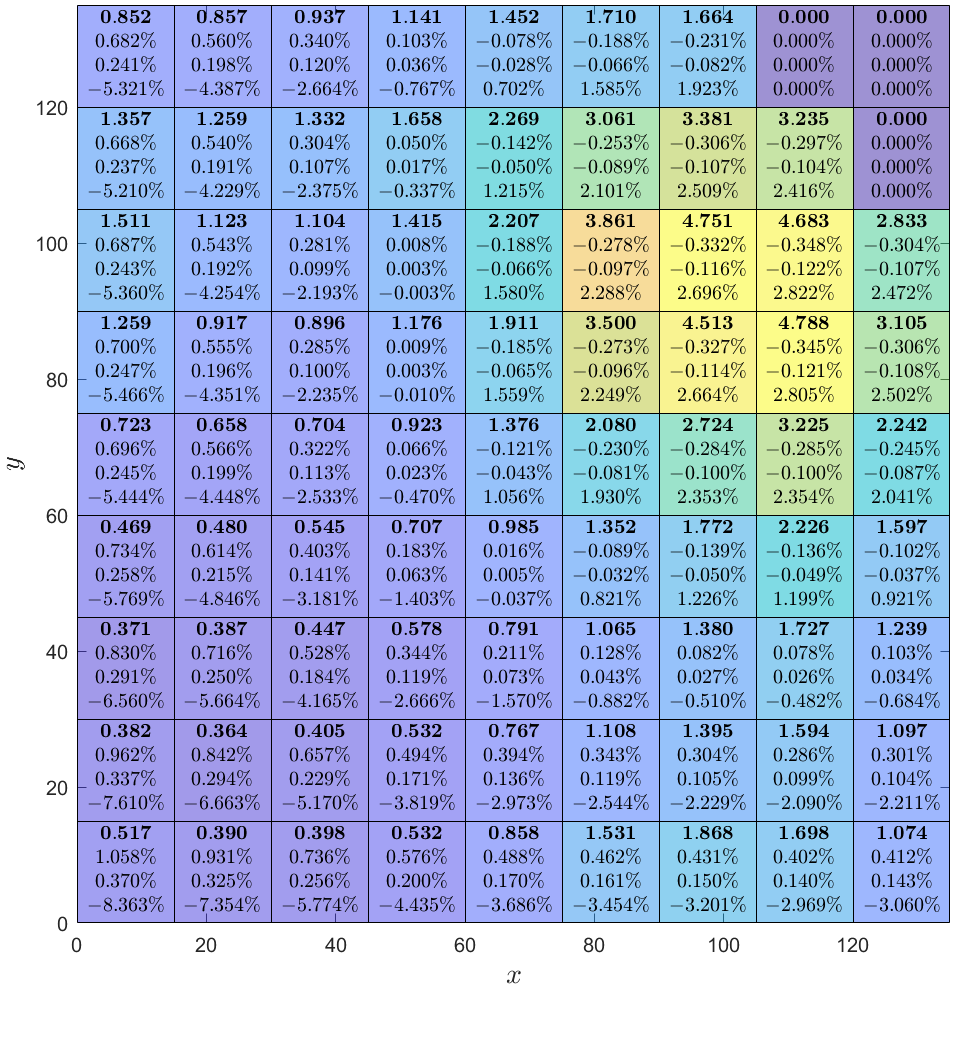
\includegraphics[height=5in]{figures/lra_block.png}};
%\node[rectangle, draw, align=center,anchor=north east, style={font=\footnotesize}] (des) at (1,0) {\textbf{Normalized Power (Ref.)} \\ Difference (IQS) - $\Delta t = 0.004, \ N_T = 4$ \\ Difference (IQS P-C) - $\Delta t = 0.004, \ N_T = 4$ \\ Difference (Implicit Dis.) - $\Delta t = 0.004$};
%\node[anchor= north west] (dif) at (1,0) {Difference $= \frac{\text{Power}^\text{ref} - \text{Power}}{\text{Power}^\text{ref}}$};
%
%\end{tikzpicture}%
%}

\item[\done] \medm{  Whenever errors are computed, baseline calculations are performed. How do the authors know that these baseline calculations are accurate enough to measure the error w.r.t. them? }
\begin{itemize}
\item Page 18: Added ``It should be noted that the baseline for these error computations was performed using an adaptive method for the flux equations with a tight tolerance. The proper convergence rates seen by the methods with coarser time steps show that this baseline is accurate enough for computing error."
\item Page 20: Added ``The baseline was computed using the BDF2 scheme on the flux equation with a time step of $10^{-5}$. The proper error convergences show that this solution is accurate enough to compare to for error computation for most of the convergence data points. Smallest time step scheme for IQS shows a break in the linearity of the convergence."
\end{itemize}

\end{itemize}

\section*{Minor Issues}

\begin{itemize}

\item[\done] \easy{ Page 1: ``… the amplitude, and a space- and time-dependent component, the shape [1,2,3,4,5]". What about energy? }
\begin{itemize}
\item Page 1: ``IQS involves factorizing the neutron flux solution into a time-only-dependent component, the amplitude, and a full phase-space component, the shape."
\end{itemize}

\item[\done] \easy{ Is $\phi^g$ the scalar flux or scalar flux moments in Eq 1a? }
\begin{itemize}
\item Page 3: ``Note that $\phi^g$ for neutron transport is the angular neutron flux ($\phi^g(\vec r, \vec\Omega, t)$), while for neutron diffusion it is scalar flux ($\phi^g(\vec r, t)$)."
\end{itemize}

\item[\working] \easy{ All quantities in Eq. 1a and 1b need to be defined. }
\begin{itemize}
\item Page 4: Created a table of the operator definitions (Table 1)
\end{itemize}

\item[\done] \easy{ Eq. 3a: $S_d^g$ is not defined. }
\begin{itemize}
\item Page 4: See Table 1
\end{itemize}

\item[\done] \easy{ For the uninitiated reader the term phase-space domain may not be familiar. The authors could introduce the term phase space. IQS may be interesting for people in other fields. }
\begin{itemize}
\item Page 1: ``In neutron transport, the neutron flux solution lives in a seven dimensional phase-space, dependent on time, space, energy, and direction. The neutron diffusion equation reduces this phase-space by eliminating direction."
\end{itemize}

\item[\done] \easy{ Algorithm in section 2.1 on page 5. Step 2: ``linearly interpolate". It is later stated that interpolation of higher order is done for high order schemes. }
\begin{itemize}
\item Page 5: Removed linearly from step 2
\item Page 6: ``It should be noted that Step 2 of the process generally involves a linear interpolation; however, for greater than second order shape discretizations, a higher-order interpolation is necessary."
\end{itemize}

\item[\nofix] \easy{ For the Linf nor of the shape: why is the maximum difference over the maximum value used and not the maximum relative difference ($1 - \phi^{k+1}/\phi^k$). }
\begin{itemize}
\item Included the reference for this error estimation.
\end{itemize}

\item[\done] \medm{ Eq (11) is restated in Eq (24). Why not just make Eq. 11 more general. Also, in Eq. (24) cp(T(t)) and originally the heat equation reads d(rho * cp(T) * T). Hence, the cp(T) cannot be pulled out so Eq. (24) is incorrect. }
\begin{itemize}
\item Page 8: ``For the purposes of this derivation, the adiabatic model, given in Eq. (11), has linear heat capacity. However, a nonlinear heat capacity can easily be implemented with a iterative procedure."
\item Page 28: Put $\rho C_p(T)$ inside the derivative 
\end{itemize}

\item[\done] \easy{ Figure 2. uses the delta t / 3 step that was claimed to be only for illustration purposes in Fig. 1. }
\begin{itemize}
\item Page 10: Included the variable $N_{T}$ in Figure 2
\item Page 9: $N_T$ is the number of temperature updates per macro step.
\end{itemize}

\item[\done] \medm{ Statement page 9: ``Furthermore, a very accurate representation of p(t) over the macro step is available from the PRKE solve…". I think it should be precise or else one would have to show that the equations are solved accurately. Second, what does ``very accurate" mean, ``very accurate" is comparison to what? }
\begin{itemize}
\item Page 11: ``Furthermore, a highly refined representation of $p(t)$ over the macro step is available from the PRKE solve (micro time scale). Using this fine scale information yields a more precise integration of amplitude than assuming an interpolation of the amplitude between macro step points."
\end{itemize}

\item[\done] \medm{ Implementation uses code specific jargon: kernels, auxkernels, Transient executioner, user-object. These need to be explained or cast in more general terms. }
\begin{itemize}
\item Page 13:
\begin{itemize}
\item Kernel - Evaluation of the weak-form residual for a particular piece of physics.
\item Executioner - Establishes the type of simulation. The Transient type moves the simulation in time conducting spatial evaluations at each step.
\item Auxiliary variable and kernel - ``Optional" variables that live on the same mesh as the solution and are computed algebraically using auxiliary kernels. 
\item Postprocessor - Computes scalar values over the entire spatial mesh, usually involves integrated quantities.
\item User-object - A generic type of postprocessor that allows connectivity of relevant quantities between different MOOSE objects.
A more detailed and comprehensive description of MOOSE objects can be found in [18]
\end{itemize}
\end{itemize}

\item[\done] \easy{ Page 13 top of the page ``looping over cells to evaluate", what cells, mesh cells? }
\begin{itemize}
\item Page 14: ``The PRKE parameters are written as user-objects, looping over spatial mesh cells to evaluate them."
\end{itemize}

\item[\done] \easy{ LRA benchmark: the number of elements makes no sense 11x11 = 121 and when using five uniform refinement steps one would end up with 123,904 elements. }
\begin{itemize}
\item Page 22: Fixed it to 123,904 elements, number of nodes was originally correct
\end{itemize}

\item[\done] \easy{ LRA benchmark description does not state what equations are solved, if that is provided in the ANL benchmark book it should be made clear. Equations could also be stated directly. }
\begin{itemize}
\item  Page 22: ``The equations being solved are explicitly defined in problem 14-A1 of the ANL Benchmark Problem Book [20]"
\end{itemize}

\item[\done] \easy{ In plots where delta t is plotted on the x-axis, it should be made clear that it is the macroscopic time step. }
\begin{itemize}
\item Page 14 and 22: ``Note that any instance of $\Delta t$ in the following figures and commentary signifies the size of the macro time step."
\end{itemize}

\item[\done] \easy{ Conclusions, page 27: incomplete sentence ``IQS showed expected error convergence up". }
\begin{itemize}
\item Page 31: ``...through fourth-order time discretization of the shape"
\end{itemize}

\item[\nofix] \easy{ Timing estimates for LRA: the author should make clear how they execute the LRA problem, i.e. number of processors and processor model. Given the long runtimes, it appears that a single processor is used. Is this to avoid problems with asynchronous behavior in parallel? }
\begin{itemize}
\item Already stated on Page 24: ``These run-times are based on total alive time of the execution where the diffusion evaluation is distributed over 24 processors."
\end{itemize}

\end{itemize}

\section*{Bibliography}

\begin{itemize}

\item[\done] \easy{ MOOSE reference is out of date. Recommend newer publication }
\begin{itemize}
\item See [16]
\end{itemize}

\item[\done] \easy{ Rattlesnake reference [17] is out of date. Recommend citing the theory manual INL/EXT-17-42103. }
\begin{itemize}
\item See [17]
\end{itemize}

\item[\done] \easy{ The LRA benchmark is extensively discussed in the Rattlesnake user manual, which might be a handy reference to use: INL/EXT-15-37337. }
\begin{itemize}
\item Page 22: ``The execution of the benchmark was performed by the Rattlesnake/MOOSE framework at Idaho National Laboratory (INL) [25]"
\end{itemize}

\end{itemize}


\end{document}